\section{Optimization with Multivariable Functions}
\label{sec:multi-opt}

The partial derivatives tell us something about where a surface has local maxima and minima. Remember that even in the one-variable cases, there were critical points which were neither maxima nor minima – this is also true for functions of many variables. In fact, as you might expect, the situation is even more complicated.

\subsection{Second Derivatives}
When you find a partial derivative of a function of two variables, you get another function of two variables – you can take its partial derivatives, too. We've done this before, in the one-variable setting. In the one-variable setting, the second derivative gave information about how the graph was curved. In the two-variable setting, the second partial derivatives give some information about how the surface is curved, as you travel on cross-sections – but that's not very complete information about the entire surface.

Imagine that you have a surface that's ruffled around a point, like what happens near a button on an overstuffed sofa, or a pinched piece of fabric, or the wrinkly skin near your thumb when you make a fist. Right at that point, every direction you move, something different will happen – it might increase, decrease, curve up, curve down… A simple phrase like concave up or concave down can't describe all the things that can happen on a surface.

Surprisingly enough, though, there is still a second derivative test that can help you decide if a point is a local maximum or minimum or neither, so we still do want to find second derivatives.

\begin{definition}[Second Partial Derivatives]
Suppose $f(x,y)$ is a function of two variables. Then it has four {\bf second partial derivatives}\index{Derivative!second partial}\index{Second partial derivative}:
$$f_{xx} = \frac{\partial}{\partial x}(f_x) = (f_x)_x \quad f_{xy} = \frac{\partial}{\partial y}(f_x)=(f_x)_y $$
$$f_{yx} = \frac{\partial}{\partial x}(f_y) = (f_y)_x \quad f_{yy} = \frac{\partial}{\partial y}(f_y)=(f_y)_y \enspace .$$
$f_{xy}$ and $f_{yx}$ are called the {\bf mixed (second) partial derivatives}\index{Mixed partial derivative} of $f$.

Leibniz notation for the second partial derivatives is a bit confusing, and we won't use it as often.
$$f_{xx} = \frac{\partial}{\partial x}\left(\frac{\partial f}{\partial x}\right) = \frac{\partial^2 f}{\partial x^2} \quad
f_{xy} = \frac{\partial}{\partial y}\left(\frac{\partial f}{\partial x}\right) = \frac{\partial^2 f}{\partial y\partial x}$$
$$f_{yx} = \frac{\partial}{\partial x}\left(\frac{\partial f}{\partial y}\right) = \frac{\partial^2 f}{\partial x\partial y} \quad
f_{yy} = \frac{\partial}{\partial y}\left(\frac{\partial f}{\partial y}\right) = \frac{\partial^2 f}{\partial y^2}$$
Notice that the order of the variables for the mixed partials goes from right to left in the Leibniz notation instead of left to right.
\end{definition}
\begin{example}
Find all four partial derivatives of $f(x,y)=x^2-4xy+4y^2$.

\begin{solution}
  We have to start by finding the (first) partial derivatives:
\begin{align*}
f_x(x,y) &= -4x+8y \\
f_y(x,y) &=  2x-4y
\end{align*}
Now we're ready to take the second partial derivatives:
\begin{align*}
f_{xx}(x,y) &= \frac{\partial}{\partial x}(2x-4y) = 2 \\
f_{xy}(x,y) &= \frac{\partial}{\partial y}(2x-4y) =-4 \\
f_{yx}(x,y) &= \frac{\partial}{\partial x}(-4x+8y) =-4 \\
f_{yy}(x,y) &= \frac{\partial}{\partial y}(-4x+8y) =8
\end{align*}
\end{solution}\end{example}

You might have noticed that the two mixed partial derivatives were equal in this last example. It turns out that it's not a coincidence – it's a theorem!

\begin{theorem}[Mixed Partial Derivative Theorem]
  \label{thm:4-mixed}
If $f$, $f_x$, $f_y$, $f_{xy}$, and $f_{yx}$ are all continuous (no breaks in their graphs), then
$$f_{xy}=f_{yx} \enspace .$$
In fact, as long as $f$ and all its appropriate partial derivatives are continuous, the mixed partials are equal even if they are of higher order, and even if the function has more than two variables.
\end{theorem}
This theorem means that the confusing Leibniz notation for second derivatives is not a big problem -- in almost every situation the mixed partials are equal, so the order in which we compute them doesn't matter.

\begin{example}
Find $\dfrac{\partial^2 f}{\partial x\partial y}$ for $f(x,y)=\dfrac{e^{x+y}}{y^3+y}+y\ln(y)$.

\begin{solution}
  We already found the first partial derivatives in Example \ref{ex:4-partials}:
  \begin{align*}
\frac{\partial f}{\partial x} &= \frac{e^{x+y}}{y^3+y} \\
\frac{\partial f}{\partial y} &= \frac{(e^{x+y(1)})(y^3+y)-(e^{x+y})(3y^2+1)}{(y^3+y)^2}+(1)(\ln(y))+(y)\frac{1}{y}
\end{align*}
Now we need to find the mixed partial derivative. Theorem \ref{thm:4-mixed} says that $\dfrac{\partial f^2}{\partial x\partial y} = \dfrac{\partial f^2}{\partial y\partial x}$, so it doesn't matter whether we find the partial derivative of $\dfrac{\partial f}{\partial x}$ with respect to $y$ or the partial derivative of $\dfrac{\partial f}{\partial y}$ with respect to $x$. Which would you rather do?

It looks like it will be easier to compute the mixed partial by finding the partial derivative of $\dfrac{\partial f}{\partial x} = \dfrac{e^{x+y}}{y^3+y}$ with respect to $y$. It still looks messy, but it looks less messy:
$$\frac{\partial f^2}{\partial y\partial x}=\frac{\partial}{\partial y}\left(\frac{e^{x+y}}{y^3+y}\right) = \frac{e^{x+y}(y^3+y)-e^{x+y}(3y^2+1)}{(y^3+y)^2} \enspace .$$
If we had decided to do this the other way, we'd end up in the same place. Eventually.
\end{solution}\end{example}

\subsection{Local Maxima, Local Minima, and Saddle Points}
Let's briefly review optimization problems in one variable.

A {\bf local maximum}\index{Maximum!local}\index{Local maximum} is a point on a curve that is higher than all the nearby points. A {\bf local minimum}\index{Minimum!local}\index{Local minimum} is lower than all the nearby points. We know that local maximum or minimum can only occur at critical points\index{Point!critical}\index{Critical point}, where the derivative is zero or undefined. But we also know that not every critical point is a maximum or minimum, so we also need to test them, with the First Derivative or Second Derivative Test\index{First derivative test}\index{Second derivative test}.

The situation with a function of two variables is much the same. Just as in the one-variable case, the first step is to find critical points, places where both the partial derivatives are either zero or undefined

\begin{definition}[Local Maximum and Minimum]
Let $f(x,y)$ be a function of two variables that exists at a point $(a, b)$.
\begin{itemize}
  \item $f$ has a {\bf local maximum}\index{Maximum!local}\index{Local maximum} at $(a,b)$ if $f(a,b) \geq f(x,y)$ for all points $(x,y)$ near $(a,b)$.
  \item $f$ has a {\bf local minimum}\index{Minimum!local}\index{Local minimum} at $(a,b)$ if $f(a,b) \leq f(x,y)$ for all points $(x,y)$ near $(a,b)$.
\end{itemize}
A {\bf critical point}\index{Point!critical}\index{Critical point} of a function $f(x,y)$ is a point $(x,y)$ (or $(x,y,f(x,y)))$ where both the following are true:
\begin{enumerate}
  \item $f_x=0$ or is undefined, and
  \item $f_y=0$ or is undefined.
\end{enumerate}
Just as in the one-variable case, a local maximum or minimum of $f$ can only occur at a critical point.
\end{definition}
Just as in the one-variable setting, not every critical point is a local maximum or minimum. For a function of two variables, the critical point could be a local maximum, local minimum, or a saddle point.

A point on a surface is a local maximum if it's higher than all the points nearby; a point is a local minimum if it's lower than all the points nearby.

A saddle point is a point on a surface that is a minimum along some paths and a maximum along some others. It's called this because it's shaped a bit like a saddle you might use to ride a horse. You can see a saddle point by making a fist – between the knuckles of your index and middle fingers, you can see a place that is a minimum as you go across your knuckles, but a maximum as you go along your hand toward your fingers.

Figure \ref{fig:4-3-saddle} shows a saddle point of the surface $z = f(x, y) = 5x^2-3y^2+10$ from a few different angles. The saddle point is above the origin and the lines show what the surface looks like above the $x$ and $y$-axes. Notice how the point above the origin, where the lines cross, is a local minimum in one direction, but a local maximum in the other direction.

\begin{figure}
  \centering
    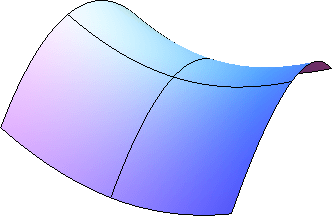
\includegraphics[width=0.4\textwidth]{img/chap4/image046.png}~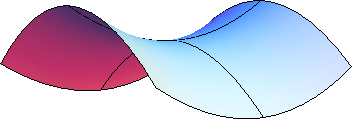
\includegraphics[width=0.4\textwidth]{img/chap4/image047.png}\\
    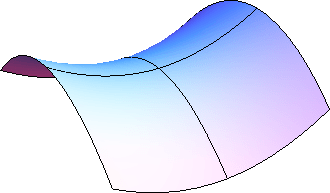
\includegraphics[width=0.4\textwidth]{img/chap4/image048.png}~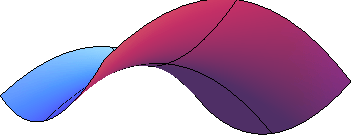
\includegraphics[width=0.4\textwidth]{img/chap4/image049.png}\\
    \caption{Saddle point of $z=f(x,y)=5x^2-3y^2+10$}
    \label{fig:4-3-saddle}
\end{figure}

\subsection{Second Derivative Test}
Just as in the one-variable case, we'll need a way to test a critical point to see whether it is a local maximum or minimum. There is a second derivative test for functions of two variables that can help, but, just as in the one-variable case, it isn't always conclusive.

\begin{theorem}[The Second Derivative Test\index{Second Derivative Test} for Functions of Two Variables]
\label{thm:4-second-deriv-test}
Find all critical points of $f(x,y)$.
Compute
$$D(x,y)=(f_{xx})(f_{yy})-(f_{xy})(f_{yx}) \enspace ,$$
and evaluate $D = D(x,y)$ at each critical point.
  \begin{enumerate}[label = (\alph*)]
    \item If $D>0$, then $f$ has a local maximum or minimum at the critical point. To see which, look at the sign of $f_{xx}$:
    \begin{itemize}
      \item If $f_{xx} > 0$, then $f$ has a local minimum\index{Local minimum} at the critical point.
      \item If $f_{xx} < 0$, then $f$ has a local maximum\index{Local maximum} at the critical point.
    \end{itemize}
    \item If $D<0$ then $f$ has a saddle point at the critical point.
    \item If $D=0$, there could be a local maximum, local minimum or neither (i.e., the test in inconclusive).
  \end{enumerate}
\end{theorem}
\begin{example}
Find all local maxima, minima, and saddle points for the function
$$f(x,y)=x^3+y^3+3x^2-3y^2-8 \enspace.$$

\begin{solution}
  First we find the partial derivatives: $f_x=3x^2+6x$ and $f_y=3y^2-6y$.

Critical points are the places where both of these are zero (neither is ever undefined): $f_x=3x^2+6x=3x(x+2)=0$ when $x=0$ or when $x=-2$. $f_y=3y^2-6y=3y(y-2)=0$ when $y=0$ or when $y=2$.

Putting these together, we get four critical points: $(0, 0)$, $(-2, 0)$, $(0, 2)$, and $(-2, 2)$.

Now to classify them, we'll use Theorem \ref{thm:4-second-deriv-test}, the Second Derivative Test. We'll need all the second partial derivatives:
$$f_{xx}=6x+6 \enspace, \quad f_{yy}=6y-6 \enspace, \quad f_{xy}=f_{yx}=0 \enspace. $$
Then
$$D(x,y)=(6x+6)(6y-6)-(0)(0)=(6x+6)(6y-6) \enspace .$$
Now look at each critical point in turn:
  \begin{itemize}
    \item At $(0, 0)$: $D(0,0)=(6(0)+6)(6(0)-6)=(6)(-6)=-36<0$, so there is a saddle point at the point $(0, 0)$.
    \item At $(-2, 0)$: $D(-2,0)=(6(-2)+6)(6(0)-6)=(-6)(-6)=36>0$ and $f_{xx}(-2,0)=6(-2)+6=-6<0$, so there is a local maximum at the point $(-2, 0)$.
    \item At $(0, 2)$: $D(0,2)=(6(0)+6)(6(2)-6)=(6)(6)=36>0$ and $f_{xx}(0,2)=6(0)+6=6>0$, so there is a local minimum at the point $(0, 2)$.
    \item At $(-2, 2)$: $D(-2,2)=(6(-2)+6)(6(2)-6)=(-6)(6)=-36<0$, so there is another saddle point at the point $(-2, 2)$.
  \end{itemize}
\end{solution}\end{example}

\begin{example}
Find all local maxima, minima, and saddle points for the function
$$z=9x^3 + \frac{y^3}{3}-4xy \enspace .$$

\begin{solution}
  We'll need all the partial derivatives and second partial derivatives, so let's compute them all first:
$$z_x = 27x^2-4y \enspace ,\quad z_y = y^2-4x \enspace, $$
$$z_{xx} = 54x \enspace , \quad z_{xy} = z_{yx} = -4 \enspace , \quad z_{yy} = 2y \enspace.$$
Now to find the critical points, we need both $z_x$ and $z_y$ to be zero (neither is ever undefined), so we need to solve this set of equations simultaneously:
\begin{align*}
z_x = 27x^2 - 4y = 0 \\
z_y =   y^2 - 4x = 0
\end{align*}
Perhaps it's been a while since you solved systems of equations. One solution method is the substitution method -- solve one equation for one variable and substitute into the other equation:
$$\begin{cases}
27x^2 - 4y &= 0 \\
y^2 - 4x &= 0
\end{cases} \rightarrow \mbox{ Solve } y^2 - 4x = 0 \mbox{ for } x = \frac{y^2}{4} \enspace ,$$
then substitute into the other equation:
\begin{align*}
27\left(\frac{y^2}{4}\right)^2 - 4y &= 0\\
\frac{27}{16}y^4 - y &= 0
\end{align*}
Now we have just one equation in one variable to solve. Factoring out a $y$ gives
$$y\left(\frac{27}{16}y^3-1\right) = 0 \enspace ,$$
so $y=0$ or $\dfrac{27}{16}y^3-1=0$, giving $y=\sqrt[3]{\dfrac{1}{27/16}} = \dfrac{\sqrt[3]{4}}{3}$.

Plugging back in to the equation $x = \dfrac{y^2}{4}$ to find $x$ gives us the two critical points: $(0,0)$ and $\left(\frac{4}{9}, \frac{4}{3}\right)$.

Now to test them. First compute
\begin{align*}
D(x,y) &= (f_{xx})(f_{yy})-(f_{xy})(f_{yx}) \\
  &= (54x)(2y)-(-4)(-4) \\
  &= 108xy-16
\end{align*}
Then evaluate D at the two critical points:
  \begin{itemize}
    \item At $(0,0)$: $D(0,0)=-16 < 0$, so there is a saddle point at $(0, 0)$.
    \item At $\left(49, \dfrac{\sqrt[3]{4}}{3}\right)$: $D\left(\dfrac{4}{9}, \dfrac{\sqrt[3]{4}}{3}\right) = 16\left(\sqrt[3]{4} - 1\right) > 0$, and $f_{xx}\left(\dfrac{4}{9}, \dfrac{\sqrt[3]{4}}{3}\right) > 0$, so there is a local minimum at the point $\left(\dfrac{4}{9}, \dfrac{\sqrt[3]{4}}{3}\right)$.
  \end{itemize}
\end{solution}\end{example}

\subsection{Applied Optimization}
\begin{example}
A company makes two products. The demand equations for the two products are given below. $p_1$, $p_2$, $q_1$, and $q_2$ are the prices and quantities for Products 1 and 2.
\begin{align*}
  q_1 &= 200 - 3p_1 - p_2 \\
  q_2 &= 150 - p_1 - 2p_2
\end{align*}
Find the price the company should charge for each product in order to maximize total revenue. What is that maximum revenue?

\begin{solution}
Revenue is still price$\times$quantity. If we're selling two products, the total revenue will be the sum of the revenues from the two products:
\begin{align*}
R(p_1,p_2) &= p_1q_1 + p_2q_2 \\
  &= p_1(200 - 3p_1 - p_2) + p_2(150 - p_1 - 2p_2) \\
  &= 200p_1 - 3p_1^2 - 2p_1p_2 + 150p_2 - 2p_2^2 \enspace .
\end{align*}
This is a function of two variables, the two prices, and we need to optimize it (just as in the previous examples). First we find critical points. The notation here gets a bit hard to look at, but hang in there – this is the same stuff we've done before.
$$R_{p_1} = 200-6p_1-2p_2  \quad \text{and}\quad  R_{p_2}=150-2p_1-4p_2.$$
Solving these simultaneously gives the one critical point $(p_1,p_2)=(25,25)$.
To confirm that this gives maximum revenue, we need to use the Second Derivative Test. Find all the second derivatives:
$$R_{p_1p_2} = -6, R_{p_2p_2} = -4, \quad \text{and}\quad  R_{p_1p_2} = R_{p_2p_1} = -2 \enspace .$$
So $D(25, 25) = (-6)(-4)-(-2)(-2)>0$ and $R_{p_1p_2}(25,25) < 0$, so this really is a local maximum.

Thus, to maximize revenue the company should charge \$25 per unit for both products. This will yield a maximum revenue of \$4375.
\end{solution}\end{example}
